\section{Parte 1:  Configurar el proyecto de equipo de Parts Unlimited.} 
\begin{itemize}
 \item  Crear proyecto y espere a que se complete el proceso.
\begin{center}
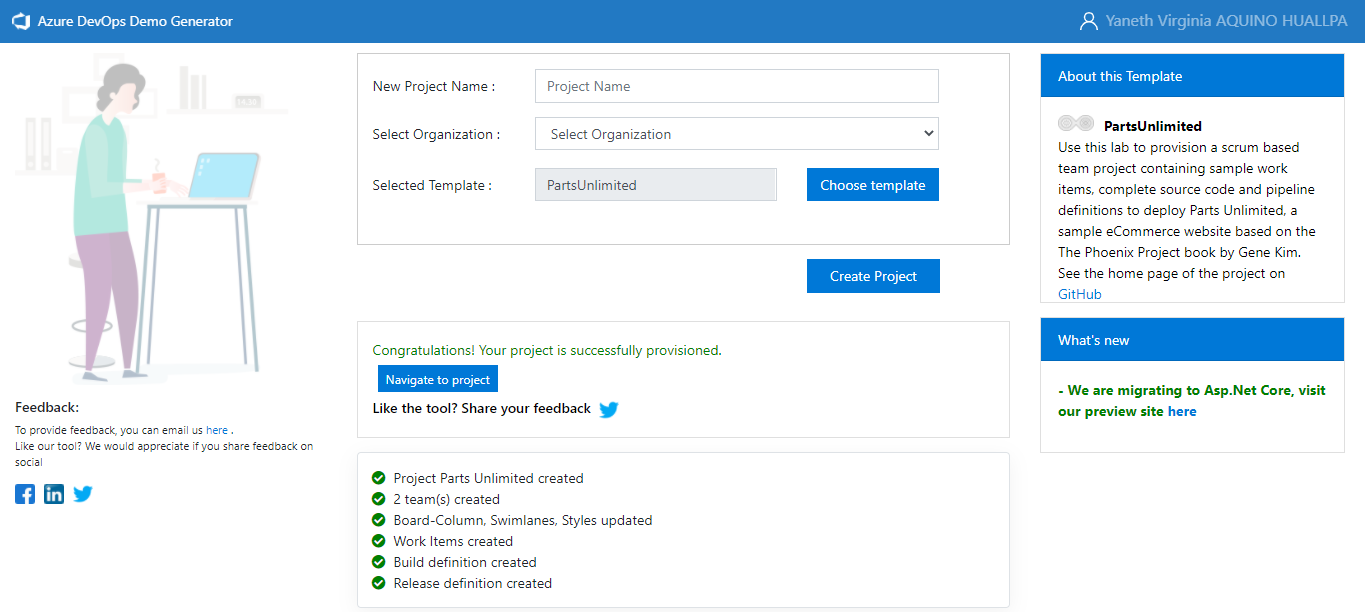
\includegraphics[width=\columnwidth]{images/1}\newline
\end{center}
 \item Configurar la solución Parts Unlimited en Visual Studio
\begin{center}
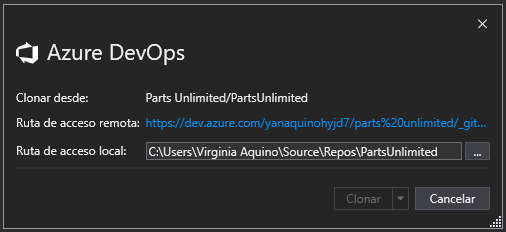
\includegraphics[width=\columnwidth]{images/2}\newline
\end{center} 
\end{itemize}

\section{Tarea 2: Comprensión de casos, conjuntos y planes de prueba} 

\begin{itemize}

\item La función principal ahora está asociada con la suite que la prueba y cualquiera puede navegar entre ellos para ver su relación en relación con los otros elementos de trabajo involucrados.
\begin{center}
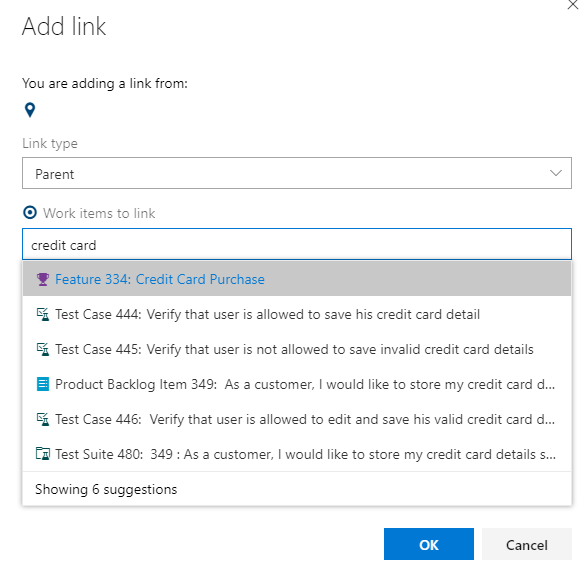
\includegraphics[width=\columnwidth]{images/4}\newline
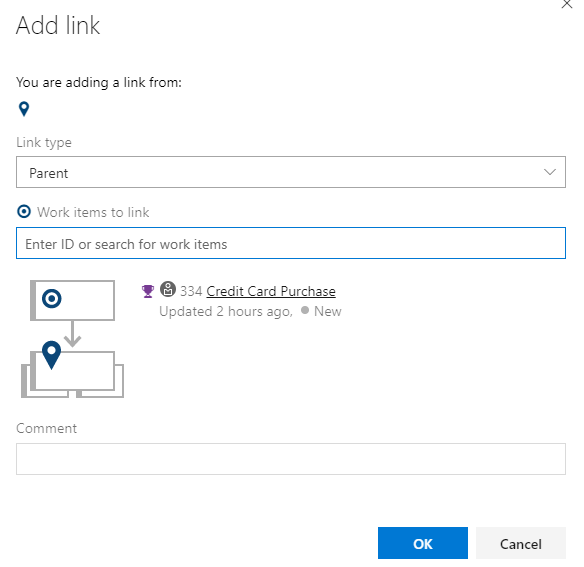
\includegraphics[width=\columnwidth]{images/6}\newline
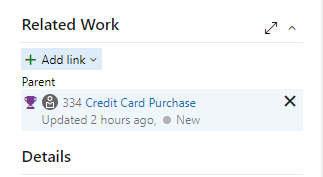
\includegraphics[width=\columnwidth]{images/7}\newline
\end{center}
\end{itemize}
\section{Tarea 3: Gestión de pruebas} 

\begin{itemize}
\item Tenga en cuenta que hay una configuración existente para Windows 10 . Cada configuración de prueba incluye un nombre y una descripción, así como un conjunto de variables de configuración personalizables . Este proyecto tiene una variable de configuración establecida para el sistema operativo . Puede agregar fácilmente más y / o editar las entradas disponibles para cada uno. Haga clic en Agregar variable de configuración .
\begin{center}
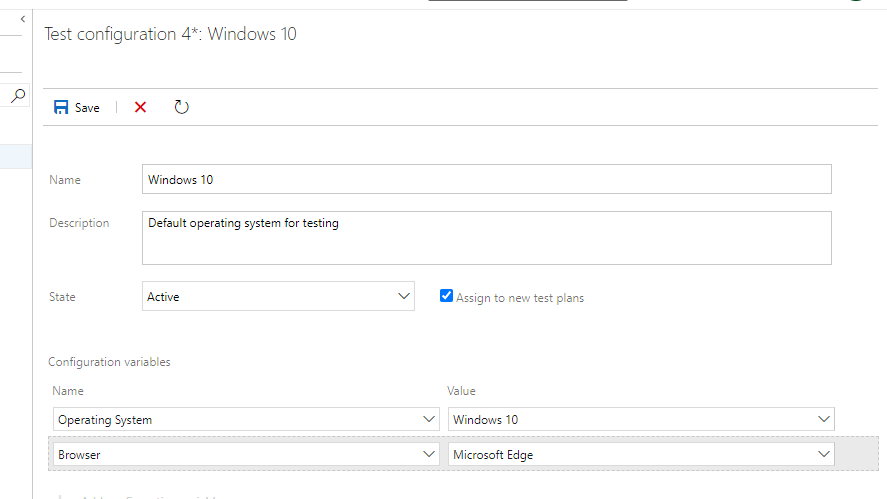
\includegraphics[width=\columnwidth]{images/10}\newline
\end{center}
\item Ahora supongamos que el equipo de prueba ha adquirido un iPhone X y quiere agregarlo a la matriz de prueba. Es realmente fácil registrar este entorno como una nueva configuración para que los casos de prueba puedan especificarlo. Sin embargo, antes de agregarlo, necesitaremos una opción de sistema operativo para iOS 10 . Haga clic en la variable de configuración del sistema operativo .
\begin{center}
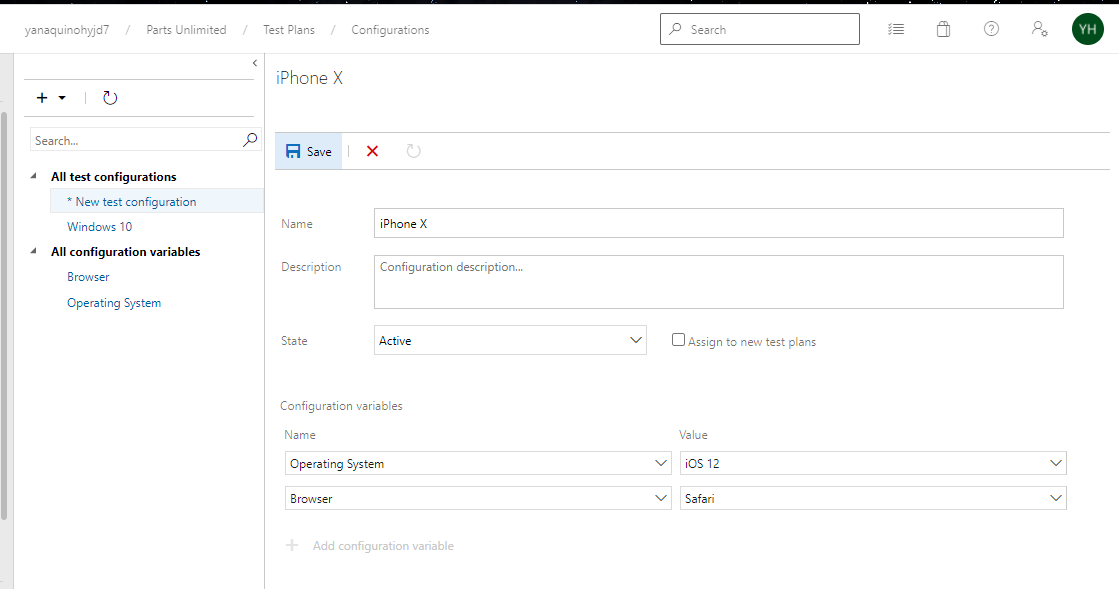
\includegraphics[width=\columnwidth]{images/13}\newline
\end{center}
\item Agregar variable de configuración dos veces y configure el navegador en Safari y el sistema operativo en iOS 12 .
\begin{center}
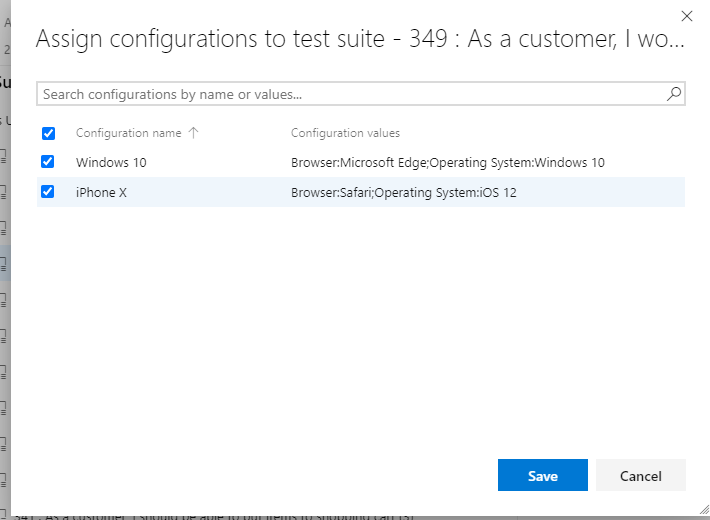
\includegraphics[width=\columnwidth]{images/14}\newline
\end{center} 
\item Tenga en cuenta que cada caso de prueba se ha duplicado con una configuración adicional para iPhone X . Ahora cada entorno se puede probar y rastrear por separado.
\begin{center}
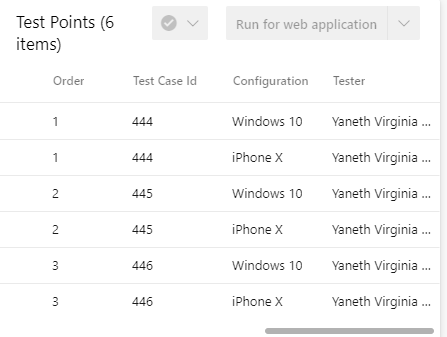
\includegraphics[width=\columnwidth]{images/15}\newline
\end{center} 
\end{itemize}

\section {Tarea 4: Autoría de pruebas } 

\begin{itemize}

\item Puede personalizar la consulta utilizada para especificar qué requisitos se recuperan, pero deje los valores predeterminados y haga clic en Ejecutar consulta . Busque y seleccione los tres elementos de la cartera de productos relacionados con el envío. Haga clic en Crear conjuntos para crear un conjunto de pruebas para cada uno.


\begin{center}
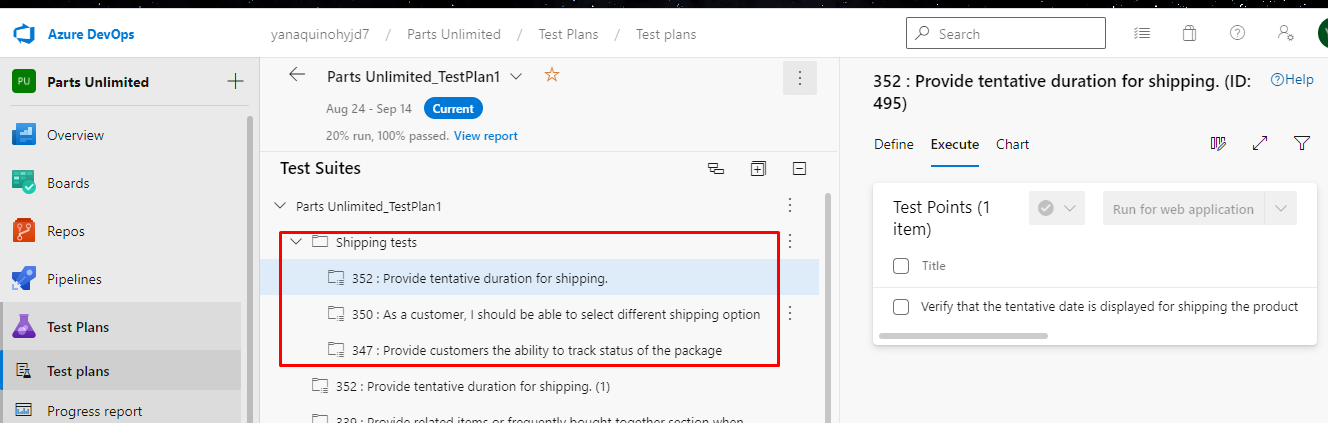
\includegraphics[width=\columnwidth]{images/16}\newline
\end{center} 
\item ngrese algunos casos de prueba y haga clic en el botón Guardar todo . El título será el título eventual del caso de prueba. Paso La acción será el primer paso (y posiblemente el único) de la prueba. Si ese paso tiene un resultado esperado, puede especificarlo como Resultado esperado del paso .
\begin{center}
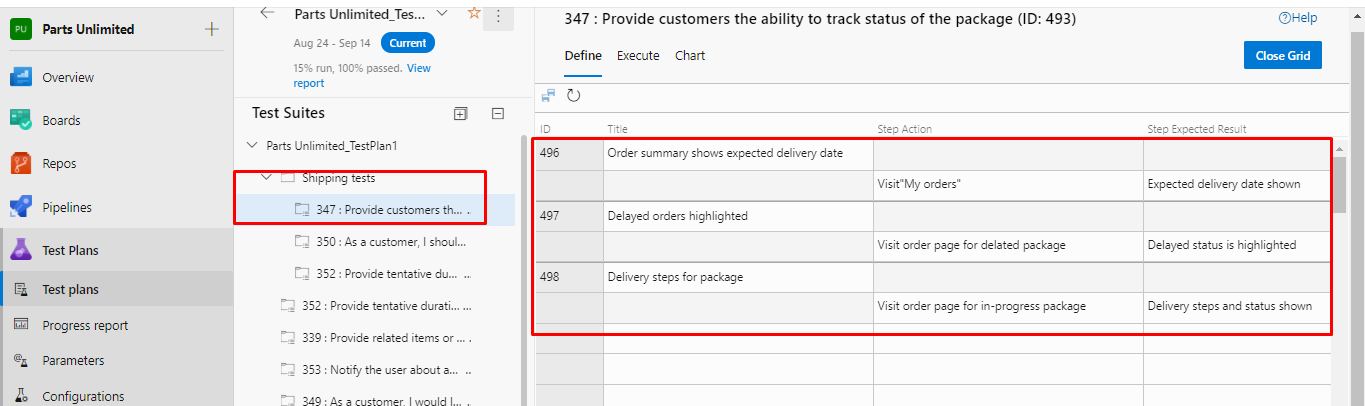
\includegraphics[width=\columnwidth]{images/17}\newline
\end{center}
\item La vista de lista muestra los mismos datos, pero en una vista diferente.
\begin{center}
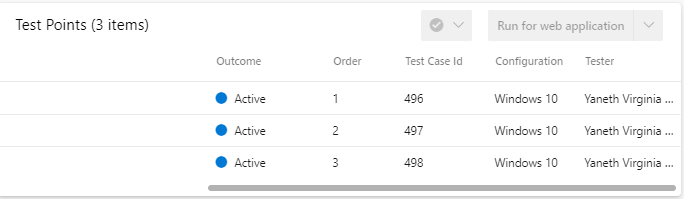
\includegraphics[width=\columnwidth]{images/19}\newline
\end{center}
\item Supongamos que desea crear un conjunto de pruebas a partir de casos de prueba relacionados con el envío en el proyecto. Cambie el Tipo de elemento de trabajo a Microsoft.TestCaseCategory para buscar casos de prueba y haga clic en Ejecutar consulta . Ahora tiene una lista de casos de prueba que puede seleccionar para crear conjuntos, si lo desea.
\begin{center}
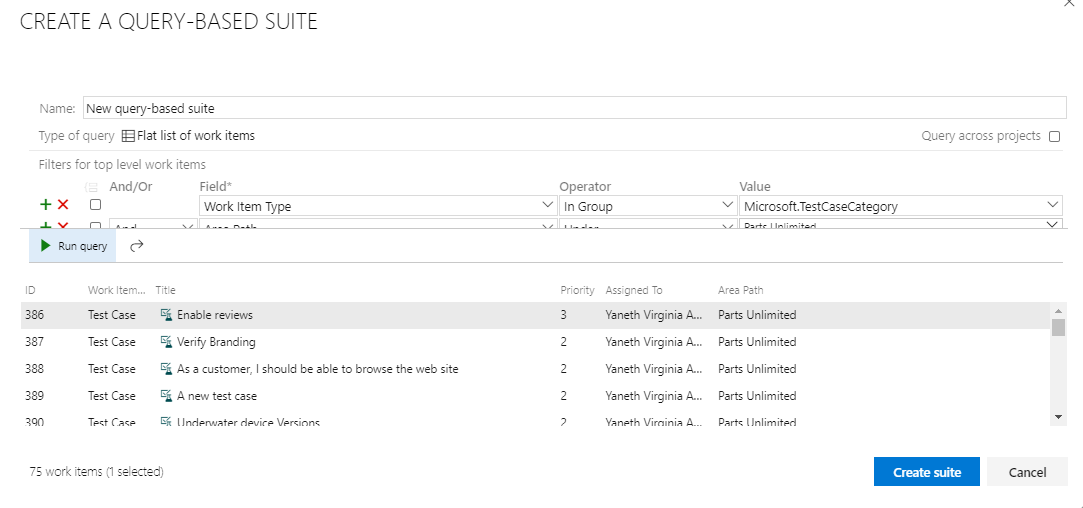
\includegraphics[width=\columnwidth]{images/18}\newline
\end{center}


\end{itemize}
\section{Ejercicio 2: creación, ejecución y análisis de pruebas manuales } 
Tarea 1: Instalar la extensión Test y  Feedback
\begin{itemize}

\item Instale Google Chrome desde http://google.com/chrome . El resto de este ejercicio utilizará Chrome como navegador. Si ya está utilizando Chrome, simplemente abra una nueva instancia para el siguiente conjunto de pasos.Vaya a Azure DevOps Marketplace en http://marketplace.visualstudio.com .Seleccione la pestaña Azure DevOps . Busque " comentarios " y haga clic en la extensión Test y Feedback .
\begin{center}
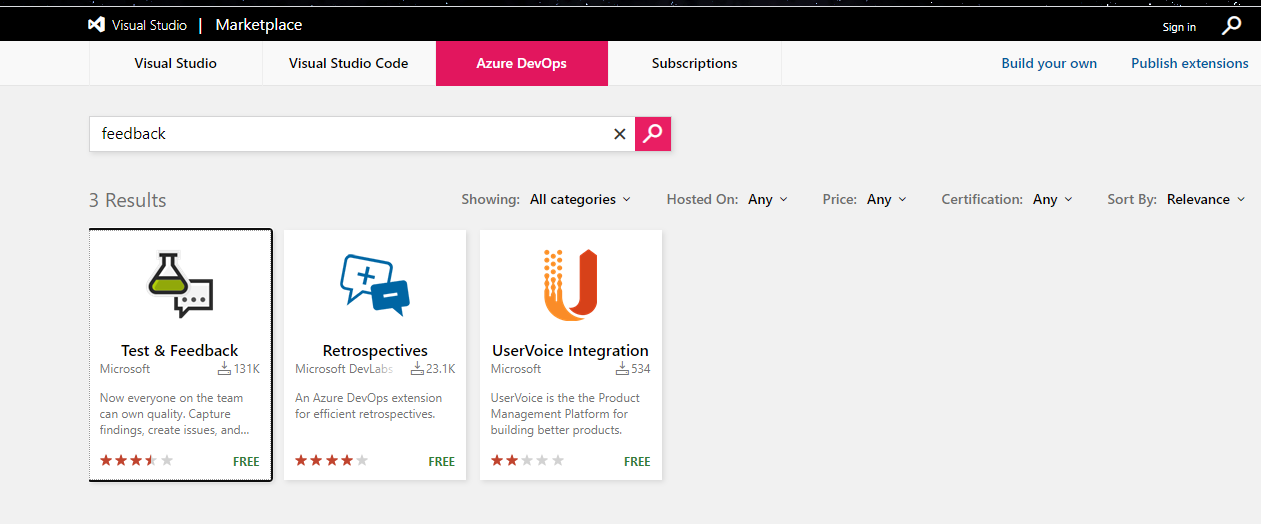
\includegraphics[width=\columnwidth]{images/20}\newline
\end{center} 
\item Instalar para la extensión de Chrome.
\begin{center}
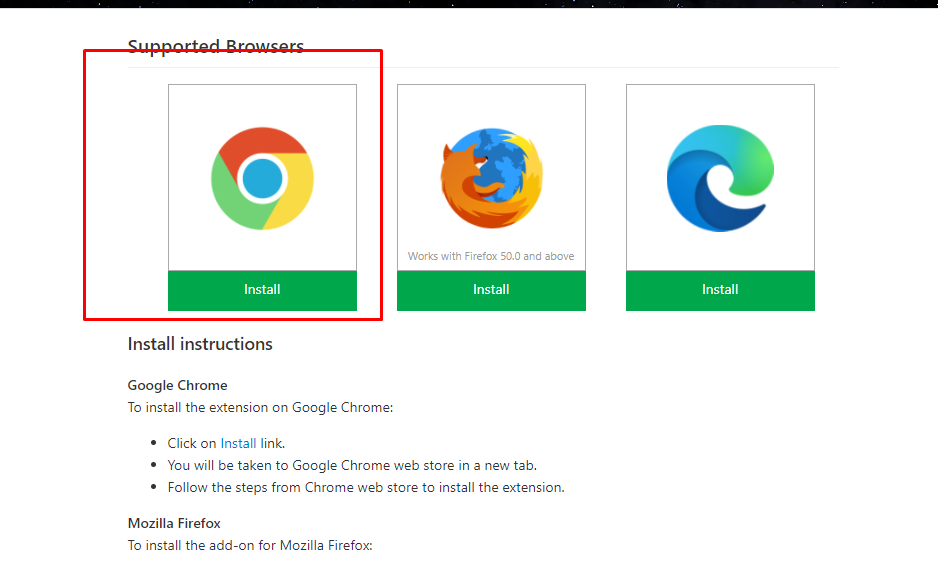
\includegraphics[width=\columnwidth]{images/21}\newline
\end{center} 
\item Para abrir la extensión, haga clic en el icono de la extensión que aparecerá a la derecha de la barra de direcciones. Seleccione la pestaña Configuración de conexión . Ingrese la URL de su instancia de Azure DevOps, como " https://MYTEAM.visualstudio.com ", como la URL del servidor y haga clic en Siguiente .
\begin{center}
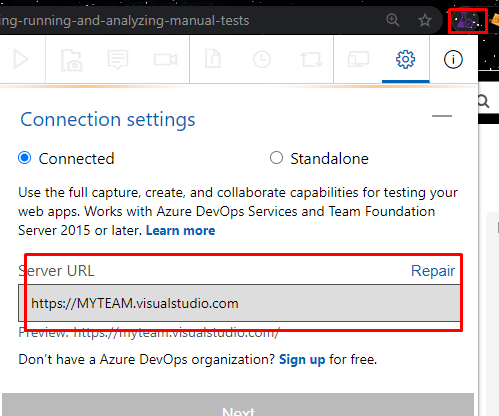
\includegraphics[width=\columnwidth]{images/22}\newline
\end{center} 
\item Después de conectarse a Azure DevOps, deberá seleccionar el equipo con el que desea asociar estos esfuerzos. Seleccione el equipo ilimitado de piezas bajo el Parts Unlimited proyecto y haga clic en Guardar para continuar.
\begin{center}
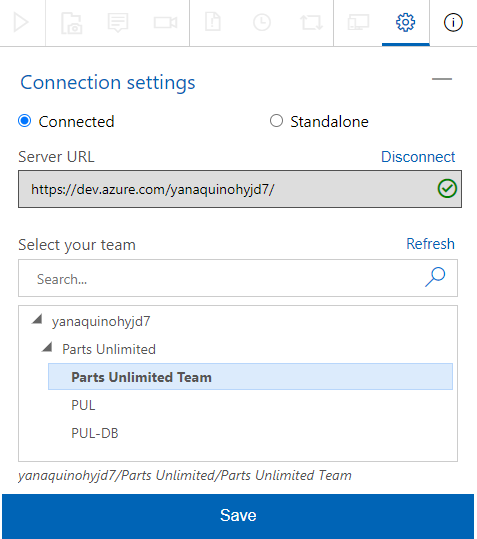
\includegraphics[width=\columnwidth]{images/23}\newline
\end{center} 

\end{itemize}

\section{Tarea 2: Creación de un plan de prueba manual } 
\begin{itemize}
\item En el cuadro Título , escriba " Confirmar que el número de pedido aparece después de un pedido exitoso " como el nombre del nuevo caso de prueba.En este punto, estamos listos para agregar pasos a esta prueba manual. Cada paso incluye una Acción , que describe la acción que el evaluador debe realizar. Opcionalmente, un paso puede incluir un resultado esperado , que describe el resultado esperado de la acción dada. En el panel Pasos , cree un paso para cada una de las siguientes acciones , de las cuales solo una tiene un resultado esperado .
\begin{center}
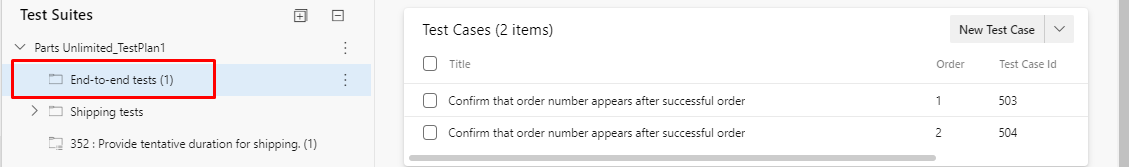
\includegraphics[width=\columnwidth]{images/32}\newline
\end{center} 
\item Para abrir la extensión, haga clic en el icono de la extensión que aparecerá a la derecha de la barra de direcciones. Seleccione la pestaña Configuración de conexión . Ingrese la URL de su instancia de Azure DevOps, como " https://MYTEAM.visualstudio.com ", como la URL del servidor y haga clic en Siguiente .
\begin{center}
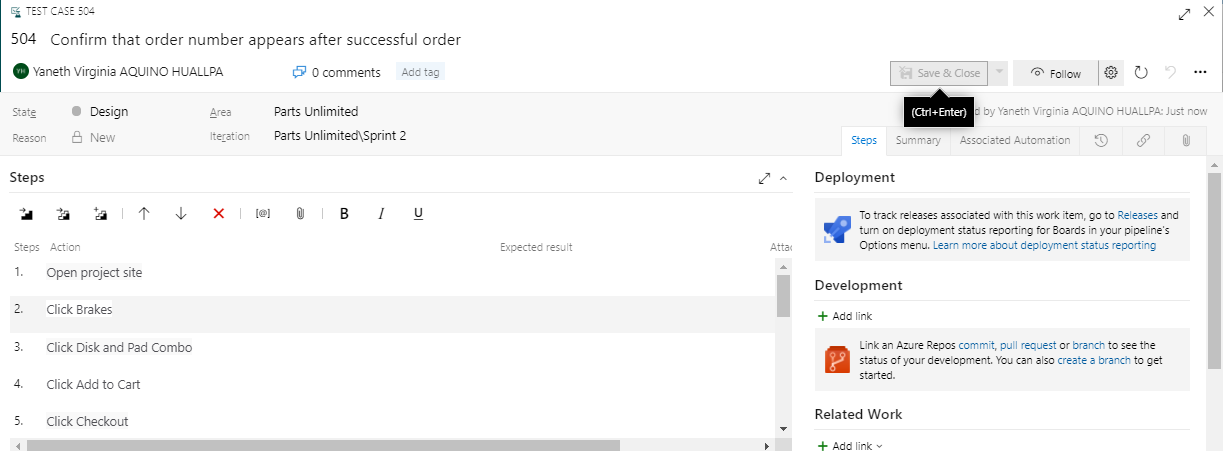
\includegraphics[width=\columnwidth]{images/30}\newline
\end{center} 
\item La sección Valores de parámetros ahora debería verse así. Tenga en cuenta que puede ingresar tantas iteraciones como necesite para probar completamente la amplitud del escenario.
\begin{center}
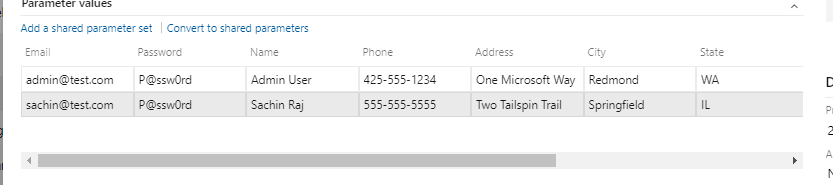
\includegraphics[width=\columnwidth]{images/31}\newline
\end{center} 

\end{itemize}
\section{Tarea 3: Ejecución de un plan de prueba manuall } 
\begin{itemize}
\item Hay algunas opciones que puede utilizar para personalizar cada ejecución de prueba. La primera opción es seleccionar un corredor , que será el navegador en este escenario. A continuación, puede tener la opción de especificar qué tipo de datos recopilar . Por último, puede especificar opcionalmente qué compilación se está probando para facilitar la asociación de los resultados con la compilación de la que proceden. Haga clic en Aceptar para continuar.
\begin{center}
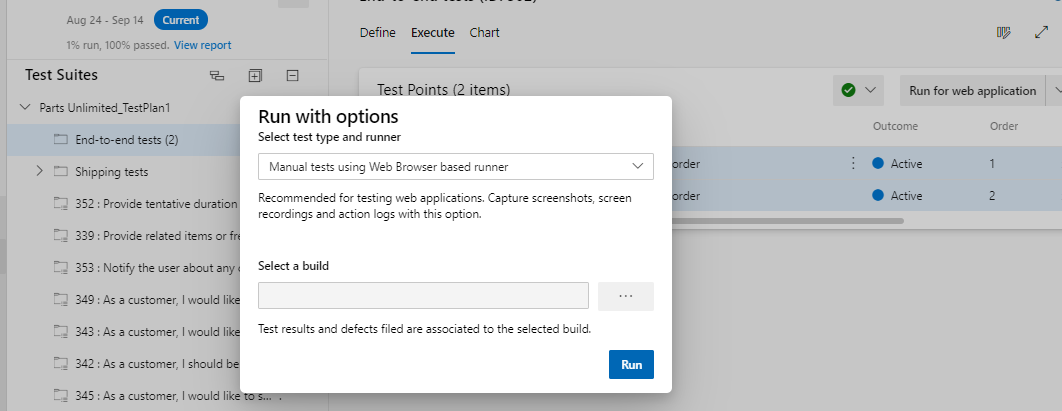
\includegraphics[width=\columnwidth]{images/40}\newline
\end{center} 
\item En la ventana Test Runner , expanda el menú desplegable Prueba 1 de 1: Iteración 1 . Tenga en cuenta que hay dos iteraciones: una para cada conjunto de parámetros especificados en el caso de prueba. En la primera iteración, se utiliza la cuenta admin@test.com . En el segundo, se utilizará sachin@test.com .
\begin{center}
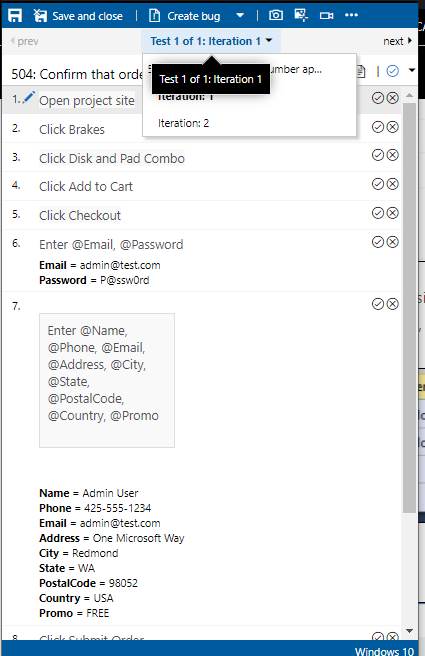
\includegraphics[width=\columnwidth]{images/41}\newline
\end{center} 
\item La sección Valores de parámetros ahora debería verse así. Tenga en cuenta que puede ingresar tantas iteraciones como necesite para probar completamente la amplitud del escenario.
\begin{center}
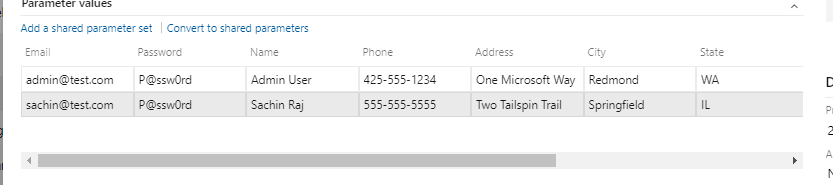
\includegraphics[width=\columnwidth]{images/31}\newline
\end{center} 
\end{itemize}



